\documentclass[a4paper,11pt,titlepage,oneside,openany]{jbook}
% \setlength{\columnsep}{2zw}

%%%%%%%%%%%%%%%%%%%%%%%%%%%%%%
% preamble
%%%%%%%%%%%%%%%%%%%%%%%%%%%%%%

%% packages
\usepackage{amsmath}
\usepackage{fancyhdr}  % pagestyle{fancy}
\usepackage[top=20truemm,bottom=20truemm,left=20truemm,right=20truemm]{geometry}
\usepackage[dvipdfmx]{hyperref,graphicx}
\usepackage{here}
\usepackage{multicol}  % for multi column
\usepackage{setspace}
\usepackage[compact]{titlesec}
\usepackage{url}
\usepackage{ulem}
% for hyperref(cf: https://ossyaritoori.hatenablog.com/entry/2016/11/11/%E3%80%90Tex%E3%80%91%E5%8D%92%E8%AB%96%E4%BF%AE%E8%AB%96%E3%81%AB%E3%81%AF%E6%98%AF%E9%9D%9E%E3%83%8F%E3%82%A4%E3%83%91%E3%83%BC%E3%83%AA%E3%83%B3%E3%82%AF%E6%A9%9F%E8%83%BD%E3%82%92%E3%81%A4)
\usepackage{pxjahyper}
\hypersetup{
	colorlinks=false, % リンクに色をつけない設定
	bookmarks=true, % 以下ブックマークに関する設定
	bookmarksnumbered=true,
	pdfborder={0 0 0},
	bookmarkstype=toc,
}
\newcommand{\linedhref}[2]{\href{#1}{\emph{#2}}}

% for check list
\usepackage{enumitem,amssymb}
\newlist{todolist}{itemize}{2}
\setlist[todolist]{label=$\square$}

%% pagestyle
% header: define for header
\pagestyle{fancy}
\lhead{}
% \chead{}
% \rhead{}

%% other
% 脚注
\renewcommand\thefootnote{\arabic{footnote})}
% フォント:cf) https://texwiki.texjp.org/?%E3%82%88%E3%81%8F%E3%81%82%E3%82%8B%E8%B3%AA%E5%95%8F#bf583189
% fix: “LaTeX Font Warning: Font shape `JY1/mc/m/it' undefined” といった警告が出る
\DeclareFontShape{JY1}{mc}{m}{it}{<->ssub*mc/m/n}{}
\DeclareFontShape{JY1}{mc}{m}{sl}{<->ssub*mc/m/n}{}
\DeclareFontShape{JY1}{mc}{m}{sc}{<->ssub*mc/m/n}{}
\DeclareFontShape{JY1}{gt}{m}{it}{<->ssub*gt/m/n}{}
\DeclareFontShape{JY1}{gt}{m}{sl}{<->ssub*gt/m/n}{}
\DeclareFontShape{JY1}{mc}{bx}{it}{<->ssub*gt/m/n}{}
\DeclareFontShape{JY1}{mc}{bx}{sl}{<->ssub*gt/m/n}{}
\DeclareFontShape{JT1}{mc}{m}{it}{<->ssub*mc/m/n}{}
\DeclareFontShape{JT1}{mc}{m}{sl}{<->ssub*mc/m/n}{}
\DeclareFontShape{JT1}{mc}{m}{sc}{<->ssub*mc/m/n}{}
\DeclareFontShape{JT1}{gt}{m}{it}{<->ssub*gt/m/n}{}
\DeclareFontShape{JT1}{gt}{m}{sl}{<->ssub*gt/m/n}{}
\DeclareFontShape{JT1}{mc}{bx}{it}{<->ssub*gt/m/n}{}
\DeclareFontShape{JT1}{mc}{bx}{sl}{<->ssub*gt/m/n}{}

% ノーブルの作成
\makeatletter
\renewcommand{\chapter}{%
  \if@openright\cleardoublepage\else\clearpage\fi
  \global\@topnum\z@
  \secdef\@chapter\@schapter}
\makeatother

% chapter などのタイトルの spacing
% テンプレ:\titlespacing{<command>}{<left>}{<before-sep>}{<after-sep>}[<right>]
% \titleformat{\chapter}{\Huge\bfseries}{\chaptername\ \thechapter}{0pt}{\vskip 20pt\raggedright}%
% Alter <after-sep> in the macro below to vary the separation after the \chapter title.
\titlespacing{\chapter}{0pt}{50pt}{\vspace{-10pt}}{\vspace{-50pt}}

%% title
\title{統計学メモ}
\author{@mathnuko}
\date{2020/02/12 〜}

%%%%%%%%%%%%%%%%%%%%%%%%%%%%%%
% document
%%%%%%%%%%%%%%%%%%%%%%%%%%%%%%

\begin{document}

\maketitle
\thispagestyle{empty}

\tableofcontents

\chapter*{はじめに}

この文書は統計学のポイントをまとめるためのノートである.\footnote{脚注サンプル}
hoge

% part1 統計学
\part{統計学}

\chapter{統計学の目的}

まず,「統計学とは何のための学問か」についてまとめる.目的を理解した上で統計学の体系について説明する.

\section{統計学とは何のための学問か?}

\subsection{「データ」とは?}

統計学は「データの要約,解釈を行うための学問」であるが,そもそも「データ」とは何かを定義しておく.ざっくり言うと「データ = 事実,資料」である.

\begin{itemize}
  \item データ・・・立論・計算の基礎となる,既知のあるいは認容された事実,資料.
\end{itemize}

自然科学の分野では,しばしば「データ」,「事実」は,「現象(研究対象)を観測した際に得られる数値」,つまり「数値データ」を指すことが多い\footnote{数値データとしては個数,長さ,体積,重さ,特定の事柄が起こった回数,時刻,続いた時間の長さなどがある.}.

また,「データ」は数値データに限らず,文字,文書なども立派な「データ」である.数値データではないデータを統計学で扱う場合には,前処理として数値データへの変換などが行われた後に利用される.

\subsection{統計学とは?}

「統計学とはどのような学問か」という問いに対するいくつかの説明を挙げておく.

\begin{itemize}
  \item 数値データの要約,解釈を行う上での理論的根拠を提供するための学問
  \item (赤本\footnote{統計学入門(東京大学出版)}の説明を要約)数値データをどのように分析し,どのような判断を下したら良いかを論ずるための学問
  \item 対象とする集団,現象の数値データからその性質,法則性を導き出すための学問
\end{itemize}

\newpage

\section{統計学の体系:記述統計学と推測統計学}

「データに対する解釈を与える」という統計学の目的を達成するためにはどうすれば良いか?\\

ある現象の法則性を導くためには,まず,現象に関するデータを観測,取得する必要がある.
ここでは,「ある現象に関するデータを観測・取得済み」の状態を考える.
それらのデータから現象の法則性を導き出すためには,以下の 2 つの手順が考えられる.

\begin{itemize}
  \item データから現象の法則性を道きび出すための方法
        \begin{itemize}
          \item 手元のデータを丹念に調べ,その特徴,性質を調べ,現象の規則性,法則を見出す.
          \item 手元のデータを用い,「論理性のある」推測により現象の規則性,法則を見出す.
        \end{itemize}
\end{itemize}


上記手順はどちらも「統計学」が扱う範疇であるが,これらはそのまま統計学の分類に対応する.
前者は「\textbf{記述統計学}」\footnote{記述統計学,descriptive statistics},
後者は「\textbf{推測統計学}」\footnote{推測統計学,inferential statistics,inductive statistics}と呼ばれる学問に分類される.
ざっくり説明すると以下のようになる.

\begin{itemize}
  \item 統計学
        \begin{itemize}
          \item 記述統計学・・・手元のデータの説明
          \item 推測統計学・・・手元のデータから推測\footnote{正確には「手元のデータから『母集団の性質』の推測」}
        \end{itemize}
\end{itemize}

記述統計学と推測統計学の関係が非常に分かりやすく描かれているのが以下の図.後に出てくる統計学の用語が挙げられているが,ここでは雰囲気を掴む.

\begin{figure}[H]
  \begin{center}
    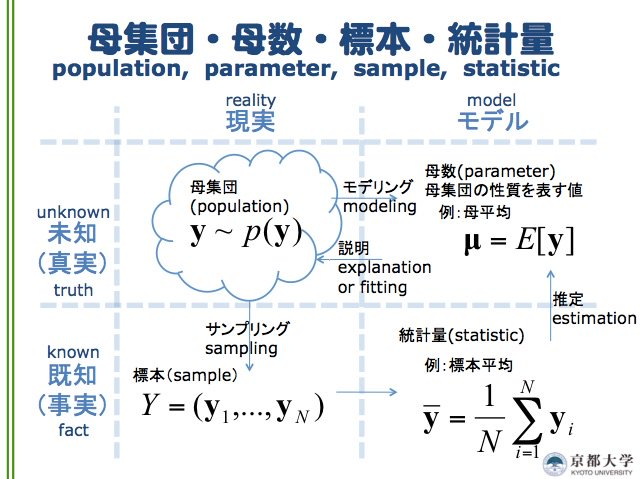
\includegraphics[width=15cm]{images/parts/1/statistics_map.jpeg}
    \caption{統計学の体系(hogeより引用)}
    % TODO: 引用元を探す
  \end{center}
\end{figure}

\section{記述統計学,推測統計学の基本的な流れ}

記述統計学,推測統計学の手法等を用いてデータ分析行う際の基本的な流れを説明する.

\subsection{データ分析における問題設定} % (fold)
\label{sub:データ分析における問題設定}

まず,データ分析の際に必ず行わなければならないのが「問題設定」である.
「〇〇という現象を理解したい」など,データ分析を行った結果何を得たいかという目的が必ず設定されているべきである.

また,\textbf{統計学はあくまでも「データに対する解釈を与える」ための手段の 1 つである},ということは認識しておくべきである.手段が目的となってはならない.
つまり,「統計学の〇〇という手法を使って△△という現象を理解したい」,「機械学習の△△という手法を使って何かできないか」ではなく,
「△△という現象を理解したい $\rightarrow$ その現象から得たデータに適した統計学(もしくは機械学習)の〇〇という手法を用いる」という順番であるべきである
\footnote{現実のデータ分析でこのような綺麗な流れがあるかは分からないが,少なくとも問題設定は必ず為されるべきである}.\\

まとめると,データ分析を行う際は,闇雲に統計学の手法を用いるのではなく,

\begin{enumerate}
  \item 「どんな現象を理解したいか」という\textbf{問題設定}
  \item 必要なデータの取得
  \item データの解釈,データから推測(必要であれば統計学の手法を用いる)
\end{enumerate}

という手順を踏むべきである.「問題設定 $\rightarrow$ データに適した統計学の手法の選択」という流れを意識したい.問題設定には例えば以下のようなものが考えられる.

\begin{itemize}
  \item 問題設定の例
        \begin{itemize}
          \item ある現象のデータからその傾向を見たい(記述統計学)
          \item 〇〇という仮説を検証したい(記述統計学,推測統計学)
          \item 手元のデータから未来のデータを予測したい(推測統計学)
        \end{itemize}
\end{itemize}

% subsection データ分析における問題設定 (end)

\newpage

\subsection{データ分析の流れ} % (fold)
\label{sub:データ分析の流れ}

前節を踏まえ,記述統計学,推測統計学の手法等を用いてデータ分析行う際の基本的な流れをざっくりまとめてみる.
両者の最終的なアウトプットの違いに着目すると良い.

\vspace{10pt}

\fbox{\parbox{\textwidth}{記述統計学の流れ
    \begin{enumerate}
      \item 問題設定,必要なデータを決める
      \item データの取得
      \item データの要約
      \item データの解釈
    \end{enumerate}
  }
}

\vspace{10pt}

\fbox{\parbox{\textwidth}{推測統計学の流れ
    \begin{enumerate}
      \item 問題設定,必要なデータを決める
      \item データの取得
      \item データから母集団の性質に当てはまる数理モデルを構築\footnote{統計モデル,時系列モデル,機械学習モデル,微分方程式モデルなど}
      \item 数理モデルを使った推定・推測・推論(データを生成する未知の真の確率分布)
      \item 数理モデルを使った推定・推測・推論の妥当性を考察・検証
    \end{enumerate}
  }
}
\vspace{10pt}

\begin{itemize}
  \item 記述統計学のアウトプット:対象となる現象,集団の性質,特徴の説明,解釈
  \item 推測統計学のアウトプット:対象となる現象,集団の性質,特徴の予測.例えば,「予測を行うための数理モデル」がアウトプットになる.この場合,「数理モデルの構築 $\rightarrow$ 検証」まで行って初めて意味を成す.
\end{itemize}


データ分析においては,上記の流れは上から下に綺麗に流れていくものではなく,上記の流れを回すである.
必要に応じて再度データ収集を行ったり,数理モデルの構築 $\rightarrow$ 検証のサイクルを回したり,といった

% subsectionデータ分析の流れ (end)

\section{補足 データの解釈:「定性的な解釈」と「定量的な解釈」}

統計学,または統計学だけでなくもっと広い意味で「データに対する解釈」を行う際に,解釈の結果として何らか(統計学で使われる指標など)の数値に落とし込むことが当たり前のように感じられるが,必ずしも数値に落とし込むことだけが「データに対する解釈」ではない\footnote{現実に統計学が使われる場面(データ分析など)では,アウトプットとして何らかの数値(指標)に落とし込むことが求められるのがほとんどだとは思いますが...}.
データに対する特徴・性質を「言葉」で表すこともできる.

\chapter{記述統計学} % (fold)
\label{cha:記述統計学}

% chapter 記述統計学 (end)

\chapter{推測統計学} % (fold)
\label{cha:推測統計学}

% chapter 推測統計学 (end)


% part2 数理統計学
%%%%%%%%%%%%%%%%%%%%%%%%%%%%%%
% 数理統計
%%%%%%%%%%%%%%%%%%%%%%%%%%%%%%

\part{数理統計}

\chapter{正規分布の導出}

% part3 生物統計学
%%%%%%%%%%%%%%%%%%%%%%%%%%%%%%
% 生物統計のまとめ
%%%%%%%%%%%%%%%%%%%%%%%%%%%%%%

\part{生物統計学}

\chapter{生物統計学:基本}

生物統計学の基本を扱う.

\section{理解度チェックリスト}

生物統計学の基本の理解度チェックリスト\cite{キホンのキ}を以下に示した.

\begin{itemize}
  \item 基本
        \begin{todolist}
          \item 記述統計学と推測統計学の違いは?
          \item 母集団を意識して研究しているか?(研究者の基本)
          \item 母集団と標本の違いは?
          \item 母数とは?
          \item 統計量とは?
          \item 3 種類の標準偏差の違いは?
          \begin{itemize}
            \item 母標準偏差(母分散)
            \item 標本標準偏差(標本分散)
            \item 不偏標準偏差(不偏分散)
          \end{itemize}
        \end{todolist}
  \item 標本分布,推定,検定
        \begin{todolist}
          \item 標本分布とは?
          \item 標準偏差(SD)と標準誤差(SE)はどう違うか?
          \item SD と SE はそれぞれどんな意図を持って用いられるか?
          \item 正規性の検定,糖分酸性の検定は何のためにあるのか?必要か?
          \item パラメトリック検定,ノンパラメトリック検定とは何か?どう使い分ける?
          \item 対応のある(関連した)検定と対応のない(独立した)検定はどう違うのか?\footnote{対応のある検定 paired test,対応のない検定 unpaired test}
          \item 片側検定,両側検定はどう違うのか?
          \item 有意差とはどう言う意味か?どのようにして有意差を決めるのか?
          \item 帰無仮説,対立仮説,危険率,有意水準の意味とは?
        \end{todolist}
  \item 分散分析,実験計画
        \begin{todolist}
          \item 一元配置分散分析で何が分かるのか?
          \item 3 群以上ではなぜ t 検定ではなく,多重比較なのか?
          \item 二元配置分散分析で何が分かるのか?どのような実験に使えるのか?
          \item どうすれば有意差の得られやすい実験計画が立てられるのか?
          \item 実験計画の立案に統計の知識はどうかかわるのか?
        \end{todolist}
\end{itemize}

\section{標準偏差の種類}

母標準偏差・・・母集団の平均からのずれ(ばらつき)を表す値.

\[
  \sigma = \sqrt{\frac{\Sigma(x_i - \mu)^2}{N}}
\]

標本標準偏差・・・標本の平均からのずれ(ばらつき)を表す値.

\[
  s = \sqrt{\frac{\Sigma(x_i - \bar{x})^2}{n}}
\]

不偏標準偏差・・・母標準偏差を推定するための値.

\[
  u = \sqrt{\frac{\Sigma(x_i - \bar{x})^2}{n-1}}
\]

\section{標本平均の分布}

母集団が $N(\mu, \sigma^2)$ から標本抽出を行った時,サンプルサイズを $n$,各観測値を $X_i$,観測値の平均値を $\bar{X}$,とする.各観測値は独立とする.

各観測値は $N(\mu, \sigma^2)$ に従うため,以下のように表せる.

\begin{eqnarray}
  X_1 \sim N(\mu, \sigma^2)\\
  X_2 \sim N(\mu, \sigma^2)\\
  \vdots\\
  X_n \sim N(\mu, \sigma^2)
\end{eqnarray}

各観測値は独立であるため,以下が成り立つ.

\begin{eqnarray}
  X_1 + X_2 + \cdots + X_n & \sim & N(\mu + \mu + \cdots + \mu, \sigma^2 + \sigma^2 + \cdots + \sigma^2)\\
  X_1 + X_2 + \cdots + X_n & \sim & N(n\mu, n\sigma^2)(「観測値の和」が従う確率分布)
\end{eqnarray}

上記より,標本平均 $\bar{X}$ の従う分布が導ける.

\begin{eqnarray}
  \frac{X_1 + X_2 + \cdots + X_n}{n} & \sim & N(\mu, \frac{\sigma^2}{n})(\because V(c X) = c^2 V(X))\\
  \bar{X} & \sim & N(\mu, \frac{\sigma^2}{n})
\end{eqnarray}

\newpage

\subsection{補足:期待値,分散の性質}

標本平均の従う分布を導く際に利用した期待値の性質をまとめておく.

\begin{itemize}
  \item 期待値
        \begin{eqnarray}
          E(X) & = & \sum_{i=1}^{n} x_i f(x)(離散型)\\
          E(X) & = & \int_{-\infty}^{\infty} x f(x)(連続型)
        \end{eqnarray}
  \item 期待値の演算
        \begin{equation}
          \begin{aligned}
            E(c)     & = c(定数)                     \\
            E(X + c) & = E(X) + c                      \\
            E(cX)    & = c E(X)(期待値のスカラー倍)  \\
            E(X + Y) & = E(X) + E(Y)(期待値の加法性)
          \end{aligned}
        \end{equation}
\end{itemize}

続いて分散の性質を列挙する.

\begin{itemize}
  \item 分散
        \begin{eqnarray}
          V(X) & = & E\{(X - \mu)^2\}(定義)\\
          V(X) & = & \sum_{i=1}^{n} (x_i - \mu)^2 f(x)(離散型)\\
          V(X) & = & \int_{-\infty}^{\infty} (x - \mu)^2 f(x)(連続型)
        \end{eqnarray}
  \item 分散の定義から導かれる性質
        \begin{eqnarray}
          V(X) = E(X^2) - (E(X))^2
        \end{eqnarray}

        証明
        \begin{eqnarray*}
          \begin{aligned}
            V(X) & = E\{(X - \mu)^2\}(\because 分散の定義)                                      \\
                 & = E(X^2 - 2\mu X + \mu^2)(\because 展開)                                     \\
                 & = E(X^2) - 2\mu E(X) + E(\mu^2)(\because 期待値の加法性,期待値のスカラー倍) \\
                 & = E(X^2) - 2\mu^2 + \mu^2(\because E(X) = \mu,定数の期待値)                 \\
                 & = E(X^2) - \mu^2                                                               \\
                 & = E(X^2) - (E(X))^2    (\because E(X) = \mu,定数の期待値)                   \\
          \end{aligned}
        \end{eqnarray*}
  \item 分散の演算
        \begin{eqnarray}
          \begin{aligned}
            V(c)     & = 0        \\
            V(X + c) & = V(X)     \\
            V(c X)   & = c^2 V(X)
          \end{aligned}
        \end{eqnarray}
        証明 $V(c X) = c^2 V(X)$
        \begin{eqnarray}
          \begin{aligned}
            V(c X) & = E\{(cX - E(cX))^2\}(\because 分散の定義 V(X) = E\{(X - E(X))^2\}) \\
                   & = E\{(cX - cE(X))^2\}(\because 期待値のスカラー倍)                  \\
                   & = E\{c^2(X - E(X))^2\}                                                \\
                   & = c^2 E\{(X - E(X))^2\}(期待値のスカラー倍)                         \\
                   & = c^2 V(X)(\because 分散の定義 E\{(X - E(X))^2\} = V(X))            \\
          \end{aligned}
        \end{eqnarray}
\end{itemize}

\section{標本平均の分布による区間推定}

前節では,標本平均 $\bar{X}$ が従う分布を求めることができた.これにより,「標本平均の」標準偏差が $\frac{\sigma}{\sqrt{n}}$ であることが分かった.
この「標本平均の分散」のように,ある母集団から標本抽出を行い,その観測値から得た\textbf{統計量のばらつきを標準偏差で表したもの}を「\textbf{標準誤差 standard error(SE)}」という.\\

統計量を指定せずに単に「標準誤差」と言った場合,\textbf{「標本平均の」標準誤差 stardard error of the mean(SEM)}のことを指す.

\begin{itemize}
  \item 標準誤差・・・統計量のばらつきを標準偏差で表したもの.統計量を指定せずに単に「標準誤差」と行った場合,標本平均の標準偏差(標本平均の「標準誤差」)を表すことが多い.
\end{itemize}

ここでは,標準誤差を「標本平均の標準誤差」として扱う.標準誤差は標本平均の標準偏差であるため,

\begin{itemize}
  \item 区間 $\mu \pm 1 SE$・・・標本抽出を行って標本平均を算出した時,$67 \%$ の確率でその区間に収まる
  \item 区間 $\mu \pm 1.96 SE$・・・標本抽出を行って標本平均を算出した時,$95 \%$ の確率でその区間に収まる
\end{itemize}

\newpage

\section{正規分布のグラフの概形}

正規分布 $N(\mu, \sigma^2)$ に従う母集団\footnote{正規分布に従う母集団を「正規母集団」という}から以下の条件で標本抽出を行った場合を考える.

\begin{itemize}
  \item $N(\mu, \sigma^2) = N(50, 20^2)$
        \begin{itemize}
          \item 母平均 50,母標準偏差 20(母分散 400)
        \end{itemize}
  \item サンプル数:10\footnote{サンプル数 the number of samples・・・群数,サンプルの数(\textbf{「サンプル = 群」と覚えておけば間違えない.}).詳しくは「\href{https://biolab.sakura.ne.jp/sample-size.html}{\underline{サンプル数とサンプルサイズは意味が違う}}」を参照.「サンプル」の誤用として多いのが,「個々の測定値(観測値)をサンプルと思っている」である.}
  \item サンプルサイズ:30\footnote{サンプルサイズ sample size・・・1 サンプルの大きさ.}
\end{itemize}

\begin{figure}[H]
  \begin{center}
    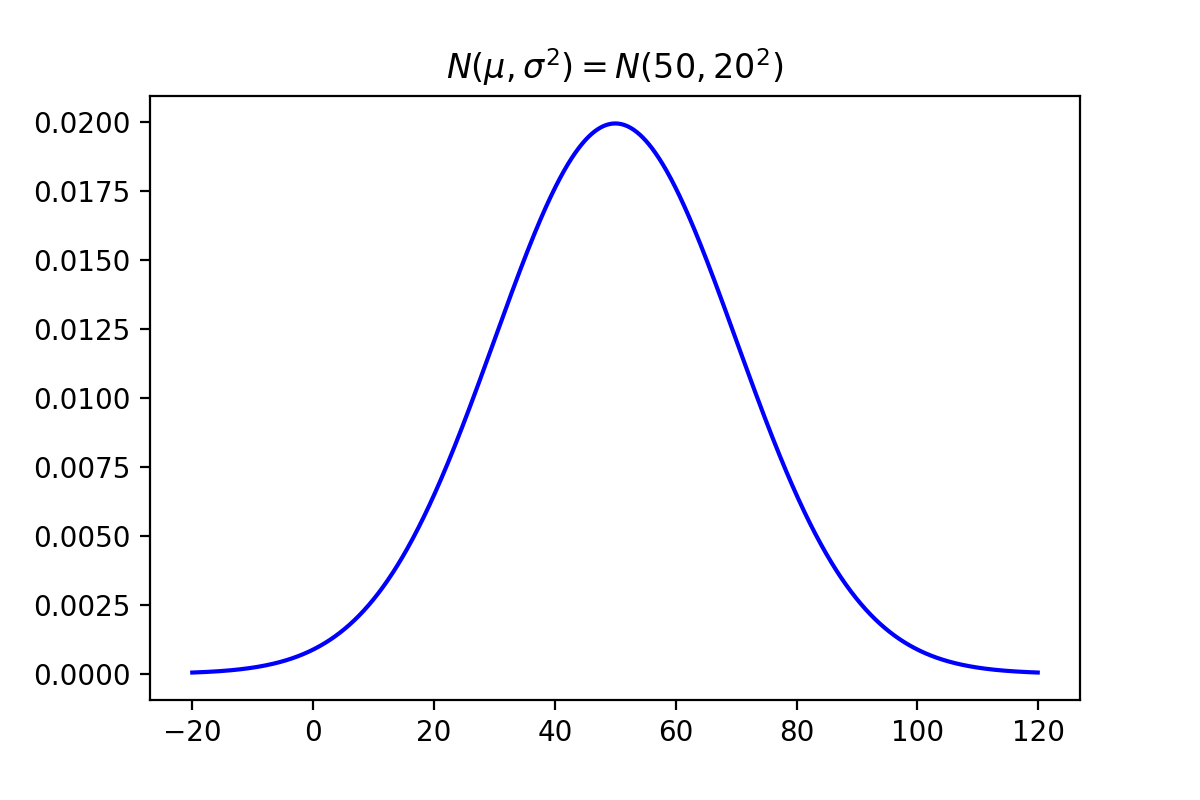
\includegraphics[width=15cm]{images/parts/3/norm-dist.png}
    \caption{$N(\mu, \sigma^2) = N(50, 20^2)$ の正規分布}
  \end{center}
\end{figure}

一つのサンプルを $X_i = \{x_1, x_2, \ldots, x_{30}\}$ としたとき,

\section{パラメトリック検定,ノンパラメトリック検定}
\section{2 群間比較の統計手法}
\section{3 群感比較の統計手法}

\chapter{生物統計学:応用}
\section{多変量解析}
\section{クラスタリング}
\section{主成分分析}

\chapter{オミクス解析}
\section{オミクス解析の基本的な流れ}
\section{トランスクリプトーム}
\subsection{Enrichment 解析}
基本,「発現が上がっている遺伝子と下がっている遺伝子の組」という発想が Enrichment 解析の精神.
「(有意に)上がっている,下がっている」をどう決めるかは関連分野の論文を参考にして定める,もしくは独自の指標で定める.

\subsection{Enrichment 解析の注意点}

GO(Gene Ontology)によって大規模データの Enrichment 解析をする時,多重検定補正をしてもなお,
補正後 p-value(q-value)は実際より高めに見積もられてしまう.
これは,各々の遺伝子に割り当てられた annotation term が重複してる場合があるためである.

「重複を免れない」というデータ構造上の問題まできちんと明示的に考えて Enrichment 解析を使ってる生物系の論文ってあまり見ない気がする.
もちろん,予め有意水準低めに設定して検定を厳しくするとかはできる.

\subsection{メタボローム}


% part4 統計学の知識のインデックス
%%%%%%%%%%%%%%%%%%%%%%%%%%%%%%
% 統計学の知識のインデックス(「統計学図鑑」)
%%%%%%%%%%%%%%%%%%%%%%%%%%%%%%

\part{統計学インデックス}

統計学図鑑\cite{統計学図鑑}を参考に,統計学のインデックスを作成する.
統計学の基礎部分の体系がどのようになっているかをざっと確認できるようにするのが目的.

%%%%%%%%%%%%%%%%%%%%%%%%%%%%%%
% chapter 統計学とは
%%%%%%%%%%%%%%%%%%%%%%%%%%%%%%

\chapter{統計学とは}

\section{統計学の分類}

統計学の分類を確認する.

\begin{itemize}
  \item 統計学・・・対象集団,現象の特徴を把握する方法を体系化した学問
        \begin{itemize}
          \item 記述統計学・・・手元のデータの特徴を捉える(平均,ばらつき,相関係数など)
          \item 推測統計学・・・手元のデータの特徴を捉える(点推定,区間推定,仮説検定)
                \begin{itemize}
                  \item 頻度論的統計学・・・一般的な統計学
                  \item ベイズ統計学(ベイズ統計学を推測統計学に含めないとする考え方もある)
                \end{itemize}
        \end{itemize}
\end{itemize}

%%%%%%%%%%%%%%%%%%%%%%%%%%%%%%
% chapter 記述統計学
%%%%%%%%%%%%%%%%%%%%%%%%%%%%%%

\chapter{記述統計学}

% section: 代表値
\section{代表値}
\subsection{平均値}
\subsection{中央値}
\subsection{最頻値}

\section{データのばらつき}
\subsection{分散,標準偏差}
\subsection{分位数}
\subsection{変動係数}

「相対標準偏差」と言われれば一発で理解できる.

\begin{itemize}
  \item 変動係数 coefficient of variattion,CV
        \begin{itemize}
          \item 標準偏差を相対化した数値.標準偏差を平均値で割ったもの.「\textbf{相対標準偏差}」ともいう.
          \item 各群の標準偏差を平均値で補正することで,\textbf{単位,平均値が異なる群間のばらつきを比較することができる.}
        \end{itemize}
\end{itemize}

\begin{align}
  CV = \frac{\sqrt{s}}{\bar{x}}
\end{align}

% section: 変量の関連性
\section{変量の関連性}

\subsection{相関係数}

\subsubsection{ピアソンの積率相関係数}

一般に,「相関係数」と言った場合「ピアソンの積率相関係数」を指すことが多い.

\subsection{順位相関係数}

\begin{itemize}
  \item 順位相関係数
        \begin{itemize}
          \item 2 つの順序変数間の相関の強さを測る指標.
                「スピアマンの順位相関係数」と「ケンドーコバヤシの順位相関係数」がある.どちらの指標を用いるかに明確な基準はない(要出典).
        \end{itemize}
\end{itemize}

\subsubsection{スピアマンの順位相関係数}

順位データに対して「ピアソンの積率相関係数」を計算した数値が「\textbf{スピアマンの積率相関係数}」である.
データが連続的な値を取る場合,まず順位データに変換する.

\subsubsection{ケンドールの順位相関係数}

%%%%%%%%%%%%%%%%%%%%%%%%%%%%%%
% chapter 確率分布
%%%%%%%%%%%%%%%%%%%%%%%%%%%%%%

\chapter{確率分布}

\section{確率変数,確率分布}

%%%%%%%%%%%%%%%%%%%%%%%%%%%%%%
% chapter 誤差論
%%%%%%%%%%%%%%%%%%%%%%%%%%%%%%

\chapter{誤差論}

\section{有効数字}
\section{系統誤差と偶然誤差}
\section{誤差の伝搬}

全ての計算を終えてから計算を行うか,間に平均などの集計を挟んで計算を行うか.
後者の場合,誤差の扱いが難しい.

%%%%%%%%%%%%%%%%%%%%%%%%%%%%%%
% chapter 推定
%%%%%%%%%%%%%%%%%%%%%%%%%%%%%%

\chapter{推定}

\section{何を「推定」するのか:母数}

推定の対象は,母数と呼ばれる母集団分布の特徴を表す定数である.

\begin{itemize}
  \item 母数 parameter
        \begin{itemize}
          \item 母集団分布の特徴を表す定数.
          \item 母平均,母分散,母標準偏差など.
        \end{itemize}
\end{itemize}



\section{統計量}
\section{統計的推測における「正規分布を仮定する」という前提}

流れの中で,今どんな前提条件,または仮定の元で論理を進めているか意識する必要がある.

\section{点推定}

母数を「1 点の数値」として推定する.
幅を持たない推定.

\subsection{推定量}
\subsection{最尤推定}
\subsection{モーメントを用いた推定}
\subsection{推定量の満たすべき性質}

\section{区間推定}

母数を「取りうる値の区間」として推定.
幅を持たせた推定.

\subsection{標本分布}

統計量が従う確率分布のこと.

\subsection{母平均の信頼区間}
\subsection{母比率の信頼区間}
\subsection{母分散の信頼区間}
\subsection{母相関係数の信頼区間}
\subsection{母相関係数の信頼区間}

\subsection{シミュレーションで母数を推定する:ブートストラップ法}
\subsubsection{ブートストラップ法}

\begin{itemize}
  \item ブートストラップ法
        \begin{itemize}
          \item 手元にある n 個のデータから同じサイズの再標本を何度も復元抽出し,その再標本の統計量から母数を推定する統計手法.
          \item 手元のデータから復元抽出を繰り返して(リサンプリング)たくさんの再標本を生成し,その統計量から母数を推定する方法.
          \item 小標本の場合など,母集団に確率分布が仮定できなくても母数の推定を可能にする.
          \item 統計学における「モンテカルロ法(コンピュータ・シミュレーション法)」の 1 つだが,乱数を用いず,実際にあるデータを使って分布を推定する.
        \end{itemize}
\end{itemize}

手元にある少ないデータだけで母数を高い精度で推定するにはどうすればいいか考えた時,

\subsubsection{母集団分布に正規性を過程できない}

区間推定では母集団分布が正規性であることを仮定することが多いが,
正規性を無理に仮定して t 分布を用いて推定しても,誤差が多すぎて実用に絶えない推定になる(信頼区間が広すぎるなど).

%%%%%%%%%%%%%%%%%%%%%%%%%%%%%%
% chapter 仮説検定
%%%%%%%%%%%%%%%%%%%%%%%%%%%%%%

\chapter{仮説検定}

\section{仮説検定とは}

帰無分布・・・帰無仮説が正しいものとして考えた時の標本分布.

\section{仮説検定の分類:パラメトリック検定とノンパラメトリック検定}
\section{帰無仮説と対立仮説}
\section{仮説検定の手順}

どのタイミングで「母集団分布」を仮定するのかに注意する.

\newpage

\section{仮説検定におけるリスク:第一種の過誤,第二種の過誤}

\subsection{第一種の過誤,第二種の過誤を図表で理解する}

どっちがどっちかややこしいけど,以下の画像を見ればすっきりする.

\begin{figure}[H]
  \begin{center}
    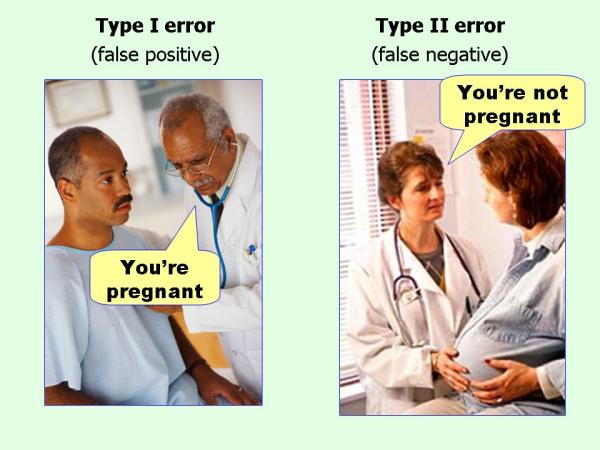
\includegraphics[width=15cm]{images/parts/4/type-i-and-type-ii-errors.jpg}
    \caption{第一種の過誤(偽陽性),第二種の過誤(偽陰性)}
  \end{center}
\end{figure}

(引用元:\linedhref{https://effectsizefaq.com/2010/05/31/i-always-get-confused-about-type-i-and-ii-errors-can-you-show-me-something-to-help-me-remember-the-difference/}{I always get confused about Type I and II errors. Can you show me something to help me remember the difference?})\\

ただ,上記画像だけでは理解が不十分.
第一種の過誤,第二種の過誤を犯してしまう際,それぞれを犯す確率というのが算出できる.
それを確率分布の図で表したものが以下.

\begin{figure}[H]
  \begin{center}
    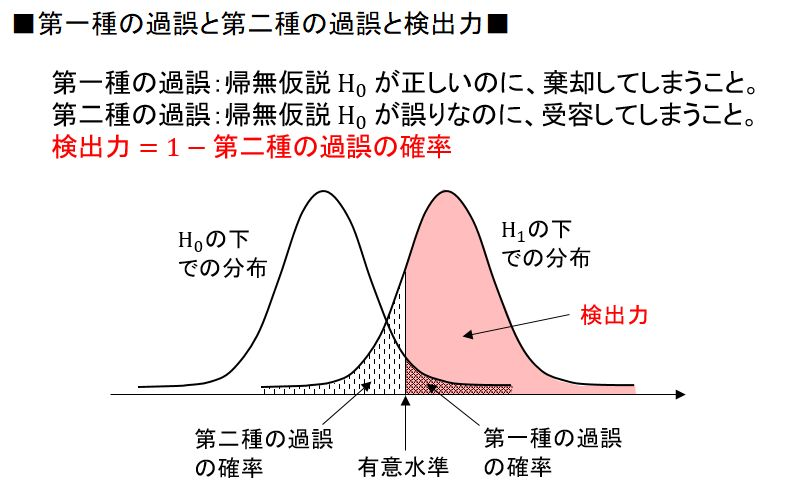
\includegraphics[width=15cm]{images/parts/4/pd-type-i-and-type-ii-errors.jpeg}
    \caption{確率分布で見る第一種の過誤(偽陽性),第二種の過誤(偽陰性)}
  \end{center}
\end{figure}

(引用元:\linedhref{https://twitter.com/ERUin2525/status/1168527197285445632}{Twitter より})\\

よく見る,第一種の過誤,第二種の過誤を整理した表は以下.
この表だけに頼ると永遠に忘れ続ける.ただし,下記画像の「差があると判断」は正しくない.
帰無仮説を「差が無い」としたとき,帰無仮説を棄却した結果主張できるのは「差が無いとは言えない」である(結果的に「差がある」と判断するだけれど)である.

(この主張↑間違っている可能性あり.「判断」だから間違いでは無い?)

\begin{figure}[H]
  \begin{center}
    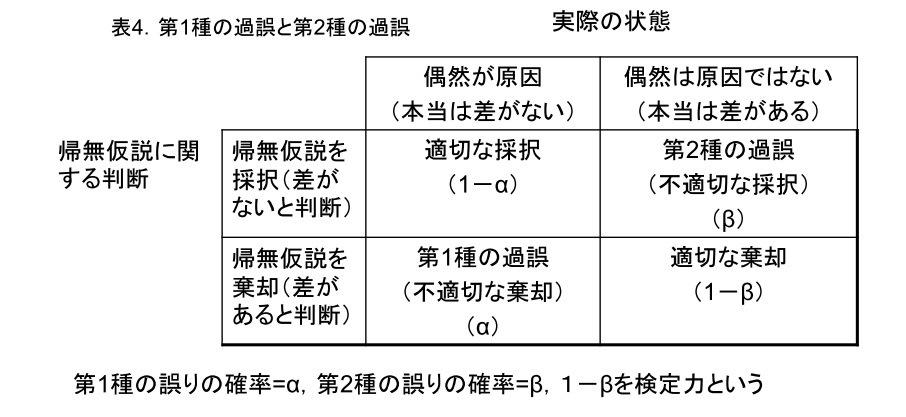
\includegraphics[width=15cm]{images/parts/4/table-type-i-and-type-ii-errors.jpeg}
    \caption{表で見る第一種の過誤(偽陽性),第二種の過誤(偽陰性)}
  \end{center}
\end{figure}

(引用元:\linedhref{https://twitter.com/kokushigou/status/529220780534411264}{Twitter より})\\

\newpage

\subsection{「第一種の過誤=有意水準」の意味するところ}

ここまでで,なぜ「第一種の過誤=有意水準(危険率)」なのかと疑問に思った.それに対する回答を以下に述べる.\\

有意水準は,「帰無分布に従うある事象が起こる確率が,有意水準より低かったら確率的に起こりにくいことであるとみなす(帰無分布から取り出される確率が低いとみなす)」という意味の(人為的な)基準である.
しかし,ある事象が起こる確率が有意水準より低くても,実は「その事象が(起こる確率は低くとも)帰無分布から発生した事象である」ということがありうる.

つまり,実際には帰無仮説が正しいのに,(人為的に決めた)棄却域に入っている値を帰無分布からサンプリングしてしまったが故に,
仮説検定によって有意だと検出されてしまったということである.

有意水準 $\alpha = 0.05$ のとき,\textbf{帰無分布からサンプリングすると $0.05$ の確率で棄却域に存在する標本を抽出してしまう}.
そして,この棄却域から抽出した標本に対して仮説検定を行うと有意だと判定されてしまう.
「実際には違うのに,有意だと判定されてしまう」,つまり,これが「偽陽性」であり,
サンプリングしたときに第一種の過誤が起こる確率が有意水準である $0.05$ そのものなのである.
「有意水準」は,第一種の過誤を起こしてしまう\emph{危険}性を数値的に示す値として「\textbf{危険率}」とも呼ばれる.

\section{母比率の検定}
\section{母分散の検定}
\section{相関の有無の判定:無相関の検定}

ただし,相関係数は「線形な」相関関係を示すものであり,「非線形な」関係の相関は表現できない.

\section{平均値の差の検定:対応のない 2 群の検定}

ほとんどの生物実験.

\section{平均値の差の検定:対応のある 2 群の検定}

マウスの血圧測定.

\section{比率の差の検定:対応のない 2 群の場合}
\section{非劣性試験}

%%%%%%%%%%%%%%%%%%%%%%%%%%%%%%
% chapter 分散分析
%%%%%%%%%%%%%%%%%%%%%%%%%%%%%%

\chapter{分散分析}

ANOVA(ANalysis Of VAriance)

\section{一元配置分散分析:実験で効果を確かめる}
\section{多群の等分散の検定:Bartlett 検定}
\section{対応のある一元配置分散分析:個体差を考慮する}
\section{二元配置分散分析:交互作用を見つけ出す}

%%%%%%%%%%%%%%%%%%%%%%%%%%%%%%
% chapter 検定の多重性
%%%%%%%%%%%%%%%%%%%%%%%%%%%%%%

\chapter{検定の多重性}

\section{検定の多重性とは}
\section{多重検定補正}
\subsection{Bonferrorni 法}

かなり厳しい多重検定補正の手法.

\subsection{Benjamini-Hochberg 法}

\linedhref{https://stats.biopapyrus.jp/stats/fdr-bh.html}{Benjamini-Hochberg 法:FDR を制御して多重比較検定補正を行う方法}

\section{Storey 法}
\section{Tukey 法,Tukey-Kramer 法}
\section{Dunnett 法}

%%%%%%%%%%%%%%%%%%%%%%%%%%%%%%
% chapter ノンパラメトリック検定
%%%%%%%%%%%%%%%%%%%%%%%%%%%%%%

\chapter{ノンパラメトリック検定}

\section{ノンパラメトリック検定:分布によらない仮説検定}

\begin{itemize}
  \item パラメトリック検定・・・母集団分布を仮定した仮説検定.
  \item ノンパラメトリック検定・・・母集団分布を仮定しない仮説検定.
\end{itemize}

\section{独立性の検定(ピアソンの $\chi^{2}$ 検定):質的データの検定}

\section{フィッシャーの正確確率検定:2 $\times$ 2 分割表の検定}
\section{対応のない 2 群の順序データの検定:マンホイットニーの U 検定}
\section{対応のある 2 群の順序データの検定:符号検定}
\section{対応のある 2 群の量的データの検定:ウィルコクソンの符号付き順位和検定}
\section{対応のない多群の順序データの検定:クラスカル・ウォリス検定}
\section{対応のある多群の順序データの検定:フリードマン検定}

%%%%%%%%%%%%%%%%%%%%%%%%%%%%%%
% chapter 実験計画法
%%%%%%%%%%%%%%%%%%%%%%%%%%%%%%

\chapter{実験計画法}

\section{フィッシャーの 3 原則:1 反復}
\section{フィッシャーの 3 原則:2 無作為化}
\section{フィッシャーの 3 原則:3 局所管理}
\section{色々な実験配置}
\section{直交計画法:実験を間引いて実施する}
\section{直交計画法の応用 1:品質工学(パラメータ設計)}
\section{直交計画法の応用 2:コンジョイント分析}

\section{検出力分析:標本サイズの決め方}
\subsection{検出力とは}
\subsection{検出力分析}

\subsection{補足:サンプルサイズとサンプル数}

\begin{itemize}
  \item サンプルサイズ,標本サイズ,sample size
        \begin{itemize}
          \item 1 標本に含まれる観測データの個数.
        \end{itemize}
  \item サンプル数,標本数,the number of samples
        \begin{itemize}
          \item 抽出した標本の数.つまり,何回標本抽出したかを表す数.
        \end{itemize}
\end{itemize}

%%%%%%%%%%%%%%%%%%%%%%%%%%%%%%
% chapter 回帰分析
%%%%%%%%%%%%%%%%%%%%%%%%%%%%%%

\chapter{回帰分析}

\section{回帰分析:原因と結果の関係を探る}
\section{最小二乗法}
\section{決定係数:回帰線の精度を評価する}
\section{t 検定:回帰線の傾きを検定する}
\section{残差分析:分析の適切さを検討する}

\section{重回帰分析:原因が複数あるときの回帰分析}
\subsection{多重共線性:説明変数間の問題}

略して「マルチコ」と呼ばれることもある.

\section{変数選択法:有効な説明変数を選ぶ}
\section{質の違いを説明する変数 1:切片ダミー}
\section{質の違いを説明する変数 2:傾きダミー}
\section{プロビット分析:2 値変数の回帰分析}
\section{イベント発生までの時間を分析する 1:生存曲線}
\section{イベント発生までの時間を分析する 2:生存曲線の比較}
\section{イベント発生までの時間を分析する 3:Cox 比例ハザード回帰}

%%%%%%%%%%%%%%%%%%%%%%%%%%%%%%
% chapter 多変量解析
%%%%%%%%%%%%%%%%%%%%%%%%%%%%%%

\chapter{多変量解析}

\section{多変量とは}

多変量データの意味から言えば,「単回帰分析」,「重回帰分析」も多変量解析に入るが,
前章で扱ったためこの章では扱わない.

\section{主成分分析:情報を縮約する}

次元削減,次元圧縮

\section{因子分析:潜在的な要因を発見する}
\section{多次元尺度構成法 MDS}
\section{クラスタリング}

神嶌先生のリンクが非常に分かりやすい.

\begin{itemize}
  \item クラスタリングの参考リンク
        \begin{itemize}
          \item \linedhref{http://www.kamishima.net/jp/kaisetsu/}{神嶌 敏弘:クラスタリング Clustering}
          \item \linedhref{http://www.kamishima.net/jp/clustering/}{クラスタリング(クラスター分析)}
        \end{itemize}
\end{itemize}

\subsection{非階層的クラスタリング}

\begin{itemize}
  \item kmeans 法
\end{itemize}

\subsection{階層的クラスタリング}

\begin{itemize}
  \item 最短距離法 nearest neighbor method
  \item 最長距離法 furthest neighbor method(完全連結法 complete linkage method)
  \item 群平均法 group average method
  \item ウォード法 Ward's method
\end{itemize}

\subsection{重要:クラスタリングの結果の解釈}

最も重要な点は,クラスタリングは探索的(exploratory)なデータ解析手法であり,クラスタリングによる分割は分析者のなんらかの主観や視点に基づいている,ということである.
よって,クラスタリングした結果は,データの要約などの知見を得るために用い,客観的な証拠として用いてはならない.

\section{構造方程式モデリング(SEM):因果構造を記述する}
\section{コレスポンデンス分析:質的データの関連性を分析する}
\section{数量化 1 類}
\section{数量化 2 類}
\section{数量化 3 類}

%%%%%%%%%%%%%%%%%%%%%%%%%%%%%%
% chapter 統計モデリング
%%%%%%%%%%%%%%%%%%%%%%%%%%%%%%

\chapter{統計モデリング}

\section{統計モデルとは}
\section{統計モデルの種類と発展}

\begin{figure}[H]
  \begin{center}
    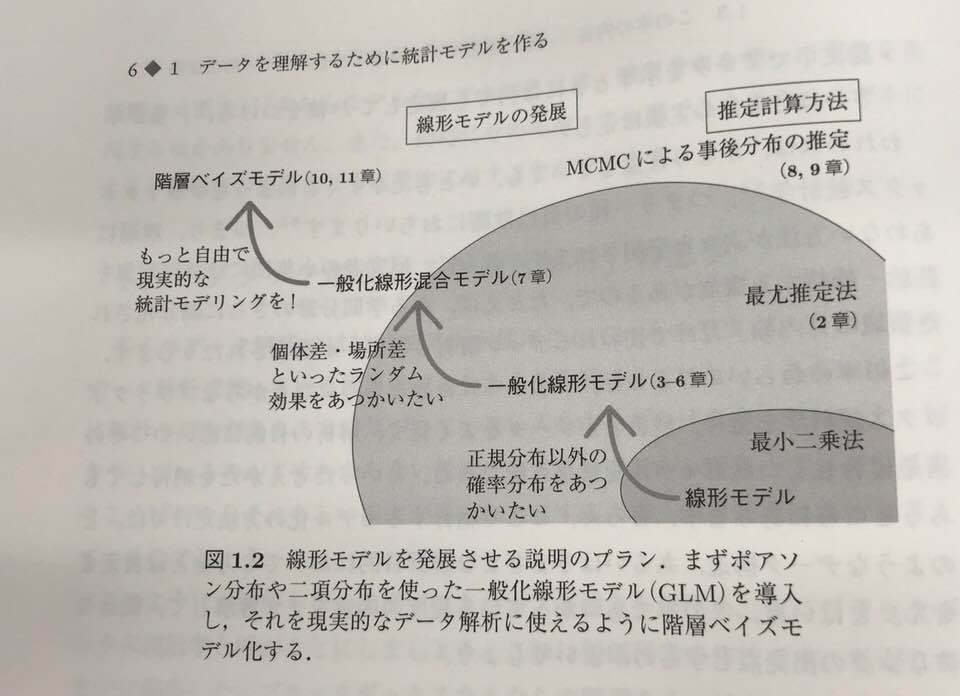
\includegraphics[width=15cm]{images/parts/4/statistical-model.jpg}
    \caption{統計モデルの発展}
  \end{center}
\end{figure}

\section{線形モデル}
\subsection{最小二乗法}

\section{一般化線形モデル}
\subsection{最尤推定法によるパラメータ推定}

\section{一般化線形混合モデル}
\section{階層ベイズモデル}

%%%%%%%%%%%%%%%%%%%%%%%%%%%%%%
% chapter 統計的因果推論
%%%%%%%%%%%%%%%%%%%%%%%%%%%%%%

\chapter{統計的因果推論}

%%%%%%%%%%%%%%%%%%%%%%%%%%%%%%
% chapter ベイズ統計学:基本
%%%%%%%%%%%%%%%%%%%%%%%%%%%%%%

\chapter{ベイズ統計学:基本}

% part5 統計検定の情報整理
%%%%%%%%%%%%%%%%%%%%%%%%%%%%%%
% 統計検定の情報の整理
%%%%%%%%%%%%%%%%%%%%%%%%%%%%%%

\part{日本統計学会 - 統計検定に関するまとめ}

\chapter{統計検定の情報の整理}

\section{統計検定 2 級}

\subsection{試験要旨}

\begin{itemize}
  \item 公式 HP:\underline{\href{https://www.toukei-kentei.jp/about/grade2/}{統計検定 2 級}}
  \item \underline{\href{https://www.toukei-kentei.jp/wp-content/uploads/grade2_hani_181214.pdf}{出題範囲}}
\end{itemize}

\newpage

\section{統計検定 1 級}

\subsection{試験要旨}

\begin{itemize}
  \item 公式 HP:\underline{\href{https://www.toukei-kentei.jp/about/grade1/}{統計検定 1 級}}
  \item \underline{\href{https://www.toukei-kentei.jp/wp-content/uploads/grade1_hani150508_2.pdf}{出題範囲}}
\end{itemize}


% reference
\bibliographystyle{jplain}
\bibliography{reference}

\end{document}